\documentclass{article}

% Document extensibility %
%
% Disables native paragraph indentation
\usepackage{parskip} 
%
% Provides further bullet options for lists
\usepackage{enumitem}

% Mathematical symbol and statement packages %
%
% Necessary
\usepackage{amsmath}
\usepackage{amssymb}
%
% Extensive fraction notation
\usepackage{xfrac}
%
% Generic mathematical commands
% Notable: \degree, \celcius
\usepackage{gensymb}
%
% Variable vector notation (arrow above variable)
\usepackage{esvect}
%
% Multiline boxed equations
\usepackage{empheq}
%
% SI Unit
\usepackage{siunitx}
%
% More intuitive arrays/matrices
\usepackage{array}
%
% Linear Equations
\usepackage{systeme}

% Graphic packages %
%
% Diagrams and illustrations
\usepackage{tikz}
\usetikzlibrary{positioning}
%
% Image insertion
\usepackage{graphicx}
\graphicspath{ {./ } }

% Document content %
%
% Change title of table of contents
% \renewcommand{\contentsname}{Title}

\title{Identifying Your Local Urban Ecological Community}
\author{Corey Mostero}
\date{27 April 2023}

\begin{document}

% Command `\hr` to insert horizontal rules
\newcommand{\hr}{\par\noindent\rule{\textwidth}{0.4pt}}

% Command to box and center math equations
\newcommand{\bc}[1]{
	\begin{equation*}
		\begin{boxed}
			{#1}
		\end{boxed}
	\end{equation*}
}

% Command for single line equations with a condition
\newcommand{\cond}[2]{
	\ifmmode
		{#1} \quad {#2}
	\else
		$$ {#1} \quad {#2} $$
	\fi
}

\maketitle
\newpage

\tableofcontents

\section{Species Identification}

\subsection{1.}
\textbf{Species Name: } Strelitzia \\
\textbf{Scientific Name: } Genus Strelitzia \\
\textbf{Common Name(s): } Bird-of-paradise flowers

\begin{enumerate}[label = \textbf{\arabic*)}]
	\item Photograph
	\item Location \\
		Outside Biology classroom
	\item Interesting Fact \\
		They are the official flower of Los Angeles, California.
	\item Observations \\
		It looks particularly unique compared to other plants with bright colors that seem to attract pollinators.
\end{enumerate}

\subsection{2.}
\textbf{Species Name: } Trachelospermum \\
\textbf{Scientific Name: } Genus Trachelospermum \\
\textbf{Common Name(s): } Star/Confederate Jasmine

\begin{enumerate}[label = \textbf{\arabic*)}]
	\item Photograph
	\item Location \\
		Area between the Mesa center, Biology classroom, and Physics classrooms.
	\item Interesting Fact \\
		All species of Trachelospermum are native to southern and eastern Asia.
	\item Observations \\
		As many of the buds were closed, it is likely that they are still yet to bloom.
\end{enumerate}

\subsection{3.}
\textbf{Species Name: } debilis \\
\textbf{Scientific Name: } Oxalis debilis \\
\textbf{Common Name(s): } Largeflower pink-sorrel

\begin{enumerate}[label = \textbf{\arabic*)}]
	\item Photograph
	\item Location \\
		Area between the Mesa center, Biology classroom, and Physics classrooms.
	\item Interesting Fact \\
		Largeflower pink-sorrels appear on every continent except Antarctica.
	\item Observations \\
		The groups of this flower seemed to bloom alongside other flowers which could either be a byproduct of the aesthetic El Camino gardeners aimed for, or a sort of biological advantage.
\end{enumerate}

\subsection{4.}
\textbf{Species Name: } Rhaphiolepis \\
\textbf{Scientific Name: } Genus Rhaphiolepis \\
\textbf{Common Name(s): } Pink Lady

\begin{enumerate}[label = \textbf{\arabic*)}]
	\item Photograph
	\item Location \\
		West of Physics department.
	\item Interesting Fact \\
		The etymology of Rhaphiolepsis comes from the Greek words \textit{rhpais}, meaning needle, and \textit{lepis}, ``the scale on the bracteole of flowers".
	\item Observations \\
		A fair amount of these flowers seemed to be wilting, which could be a consequence of the shaded area it grows in due to it being surrounded by school buildings.
\end{enumerate}

\subsection{5.}
\textbf{Species Name: } grandiflorum \\
\textbf{Scientific Name: } Linum grandiflorum \\
\textbf{Common Name(s): } Scarlet Flax

\begin{enumerate}[label = \textbf{\arabic*)}]
	\item Photograph
	\item Location \\
		The bench area between the Physics department and Cafe Camino.
	\item Interesting Fact \\
		The Scarlet Flax is native to Algeria!
	\item Observations \\
		The pollen on the Scarlet Flax seem to be relatively more visible than others.
\end{enumerate}

\subsection{6.}
\textbf{Species Name: } cyanus \\
\textbf{Scientific Name: } Centaurea cyanus \\
\textbf{Common Name(s): } Cornflower

\begin{enumerate}[label = \textbf{\arabic*)}]
	\item Photograph
	\item Location \\
		The bench area between the Physics department and Cafe Camino.
	\item Interesting Fact \\
		The Cornflower carries many myths such as how their blue color was believed to have been dyed from the sky.
	\item Observations \\
		Their bountiful and attractive palette of colors seems to be used to attract pollinators.
\end{enumerate}

\subsection{7.}
\textbf{Species Name: } sinuata \\
\textbf{Scientific Name: } Dimorphotheca sinuata \\
\textbf{Common Name(s): } Cape marigold

\begin{enumerate}[label = \textbf{\arabic*)}]
	\item Photograph
	\item Location \\
		The bench area between the Physics department and Cafe Camino.
	\item Interesting Fact \\
		Despite its beautiful and safe colors, the cape marigold is known to be an invasive plant species.
	\item Observations \\
		The orange color makes me feel like it may be flower most often in Summer.
\end{enumerate}

\subsection{8.}
\textbf{Species Name: } tanacetifolia \\
\textbf{Scientific Name: } Phacelia tanacetifolia \\
\textbf{Common Name(s): } Lacy phacelia

\begin{enumerate}[label = \textbf{\arabic*)}]
	\item Photograph

	\item Location \\
		The bench area between the Physics department and Cafe Camino.
	\item Interesting Fact \\
		Its curved stem has given it a nickname of ``scorpionweed".
	\item Observations \\
		The prickly hairs on the stem of the Lacy phacelia seems to be a means to steer pollinators to fly instead to its flower. A sort of directing mechanism.
\end{enumerate}

\subsection{9.}
\textbf{Species Name: } tinctoria \\
\textbf{Scientific Name: } Coreopsis tinctoria \\
\textbf{Common Name(s): } plains coreopsis

\begin{enumerate}[label = \textbf{\arabic*)}]
	\item Photograph

	\item Location \\
		The bench area between the Physics department and Cafe Camino.
	\item Interesting Fact \\
		Many sources claim that the name ``Coreopsis" means ``always cheerful".
	\item Observations \\
		The pattern of colors on the plains coreopsis reminds me of a bullseye, maybe used as a way to attract pollinators.
\end{enumerate}

\subsection{10.}
\textbf{Species Name: } officinale \\
\textbf{Scientific Name: } Taraxacum officinale \\
\textbf{Common Name(s): } common dandelion

\begin{enumerate}[label = \textbf{\arabic*)}]
	\item Photograph

	\item Location \\
		Between Cafe Camino and the Library.
	\item Interesting Fact \\
		Dandelions have roots that loosen soil and help prevent erosion.
	\item Observations \\
		As the picture shows the dandelion in its yellow stage, it shows that it has not yet pollinated.
\end{enumerate}

\subsection{11.}
\textbf{Species Name: } pannosa \\
\textbf{Scientific Name: } Podosphaera pannosa \\
\textbf{Common Name(s): } Rose Powdery Mildew

\begin{enumerate}[label = \textbf{\arabic*)}]
	\item Photograph

	\item Location \\
		The back side of the school library.
	\item Interesting Fact \\
		The Rose powdery mildew is said to be one of the ``most common foliar diseases of roses."
	\item Observations \\
		I found it interesting that some of the buds have flowered - greatly at that - while some were still in their bud stage. It could be inferred that their flowering stage is rather quick.
\end{enumerate}

\subsection{12.}
\textbf{Species Name: } Dietes \\
\textbf{Scientific Name: } Genus Dietes \\
\textbf{Common Name(s): } Fortnight Lilies

\begin{enumerate}[label = \textbf{\arabic*)}]
	\item Photograph

	\item Location \\
		The back side of the school library.
	\item Interesting Fact \\
		The etymology of the name ``fortnight lilies" comes from how it produces many flowers during the spring to late summer season, having only two weeks (a fortnight) of rest between each flowering period.
	\item Observations \\
		Each flower seemed to share petals with a dark brown circle in the center, possibly used as a way to scare off animals that may try to damage the flower.
\end{enumerate}

\subsection{13.}
\textbf{Species Name: } audax \\
\textbf{Scientific Name: } Phidippus audax \\
\textbf{Common Name(s): } Bold Jumping Spider

\begin{enumerate}[label = \textbf{\arabic*)}]
	\item Photograph

	\item Location \\
		The walkway from the library towards the auditorium.
	\item Interesting Fact \\
		The way jumping spiders \textit{jump}, is by changing the blood flow to their legs, where it contracts muscles in a way to fully extend them as they fly towards their target!
	\item Observations \\
		The black and white coloring of this jumping spider led me to believe that it wants to intimidate its prey by its alarming and contrasting colors.
\end{enumerate}

\subsection{14.}
\textbf{Species Name: } brachyrhynchos \\
\textbf{Scientific Name: } Corvus brachyrhynchos \\
\textbf{Common Name(s): } American Crow

\begin{enumerate}[label = \textbf{\arabic*)}]
	\item Photograph

	\item Location \\
		On top of the fence along the walkway from the library to the auditorium.
	\item Interesting Fact \\
		Crows are some of the few animals that have the intuition to make tools.
	\item Observations \\
		The crow seemed desperate and scurried often possibly meaning that it was hungry.
\end{enumerate}

\subsection{15.}
\textbf{Species Name: } Sciurus \\
\textbf{Scientific Name: } Genus Sciurus \\
\textbf{Common Name(s): } Tree Squirrels

\begin{enumerate}[label = \textbf{\arabic*)}]
	\item Photograph

	\item Location \\
		The bench area between the Physics department and Cafe Camino.
	\item Interesting Fact \\
		Squirrels utilize a unique movement tactic where the zigzag as they sprint to escape from predators.
	\item Observations \\
		The squirrel seemed eager to discover the treasures in the garbage cans, probably because it was hungry.
\end{enumerate}

\section{Food Web}

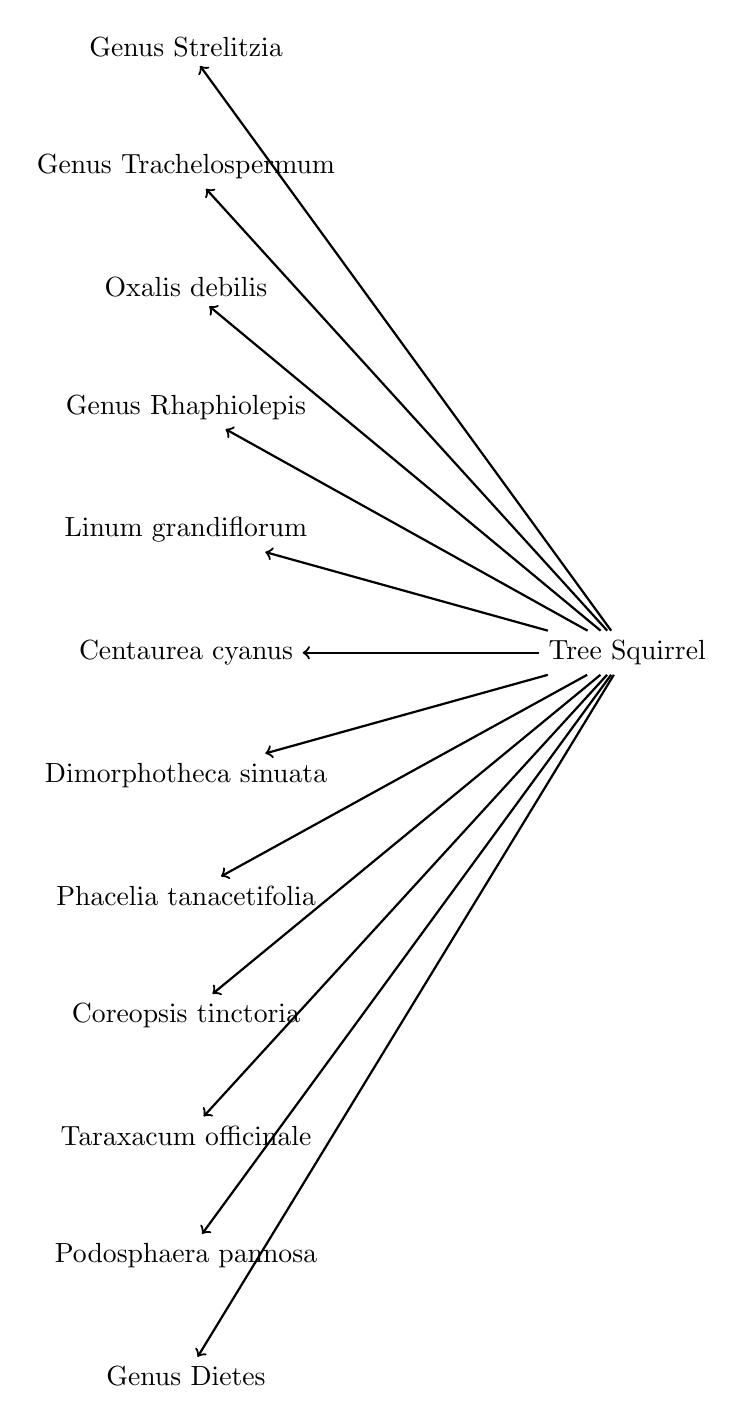
\begin{tikzpicture}
	\node (1) {Genus Strelitzia};
	\node (2) [below = of 1] {Genus Trachelospermum};
	\node (3) [below = of 2] {Oxalis debilis};
	\node (4) [below = of 3] {Genus Rhaphiolepis};
	\node (5) [below = of 4] {Linum grandiflorum};
	\node (6) [below = of 5] {Centaurea cyanus};
	\node (7) [below = of 6] {Dimorphotheca sinuata};
	\node (8) [below = of 7] {Phacelia tanacetifolia};
	\node (9) [below = of 8] {Coreopsis tinctoria};
	\node (10) [below = of 9] {Taraxacum officinale};
	\node (11) [below = of 10] {Podosphaera pannosa};
	\node (12) [below = of 11] {Genus Dietes};

	\node (squirrel) [right = 3cm of 6] {Tree Squirrel};

	\foreach \node in {1, 2, 3, 4, 5, 6, 7, 8, 9, 10, 11, 12}
		\draw[black, thick, ->] (squirrel) -- (\node);
\end{tikzpicture}

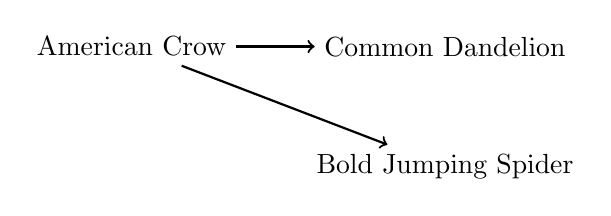
\begin{tikzpicture}
	\node(crow) {American Crow};

	\node (dandelion) [right = of crow] {Common Dandelion};
	\node (spider) [below = of dandelion] {Bold Jumping Spider};

	\draw[black, thick, ->] (crow) -- (dandelion);
	\draw[black, thick, ->] (crow) -- (spider);
\end{tikzpicture}

\end{document}
